\documentclass[12pt]{article}
\usepackage[utf8]{inputenc}
\usepackage[russian]{babel}
\usepackage{graphicx}
\usepackage{wrapfig}
\usepackage{hyperref}
\usepackage{epsf,amsmath,amsfonts,amssymb,amsbsy}
\usepackage[mathscr]{eucal}
\usepackage[left=1.5cm,right=1.5cm,
    top=2cm,bottom=2cm,bindingoffset=0cm]{geometry}
\usepackage{cmlgc}
\usepackage{array}
\usepackage{wrapfig}
\usepackage{lipsum}
\usepackage{esvect}
\usepackage{subfig}
\usepackage{calc}
\usepackage{pgfplots,tikz,circuitikz}
\usepackage{pgfplotstable}
\usepackage{tkz-euclide}

\usepackage{centernot}
\usepackage{cancel}

%Includes "References" in the table of contents
\usepackage[nottoc]{tocbibind}

\usepackage{csvsimple}


\begin{filecontents*}{data.csv}
T,U,t,y,t_new
10.154,-0.02,12.0,0.0286,11.95
10.0868,-0.02,14.02,0.0297,13.97
9.9702,-0.02,16.02,0.0319,15.97
9.8791,-0.02,17.11,0.0339,17.06
9.7815,-0.02,18.0,0.0363,17.95
9.6377,-0.02,19.01,0.0403,18.96
9.459,-0.02,20.01,0.0468,19.96
9.0662,-0.019,22.01,0.0709,21.96
8.7512,-0.02,24.02,0.1178,23.97
8.6131,-0.02,26.02,0.1642,25.97
8.5365,-0.02,28.02,0.2094,27.97
8.4882,-0.02,30.01,0.2529,29.96
8.4551,-0.02,32.0,0.2947,31.95
8.4302,-0.02,34.0,0.3364,33.95
8.4111,-0.02,36.01,0.3772,35.96
8.3966,-0.02,38.0,0.4154,37.95
8.3847,-0.02,40.0,0.453,39.95
\end{filecontents*}

\title{3.4.2}
\author{panferov.ad }
\date{September 2020}

\begin{document}

\begin{center}
  \LARGE{Работа 3.4.2}\\[0.2cm]
  \LARGE{Закон Кюри-Вейсса}\\[0.2cm]
  \large{Панферов Андрей}\\[0.2cm]
\end{center}

\section{Экспериментальная установка}
\textbf{В работе используются:} катушка самоиндукции с образцом из гадолиния, гермостат, частотомер, цифровой вольтметр, LC-автогенератор, термопара медь-константан.\\

Экспериментальная установка. Схема установки для проверки Закона Кюри Вейсса показана на рис. \ref{pic1}. Исследуемый ферромагнитный образец (гадолиний) расположен внутри пустотелой катушки самоиндукции, которая служит индуктивностью колебательного контура, входящего в состав $L C$ -автогенератора. Автогенератор собран на полевом транзисторе КП-103 и смонтирован в виде отдельного блока.

\begin{center}
    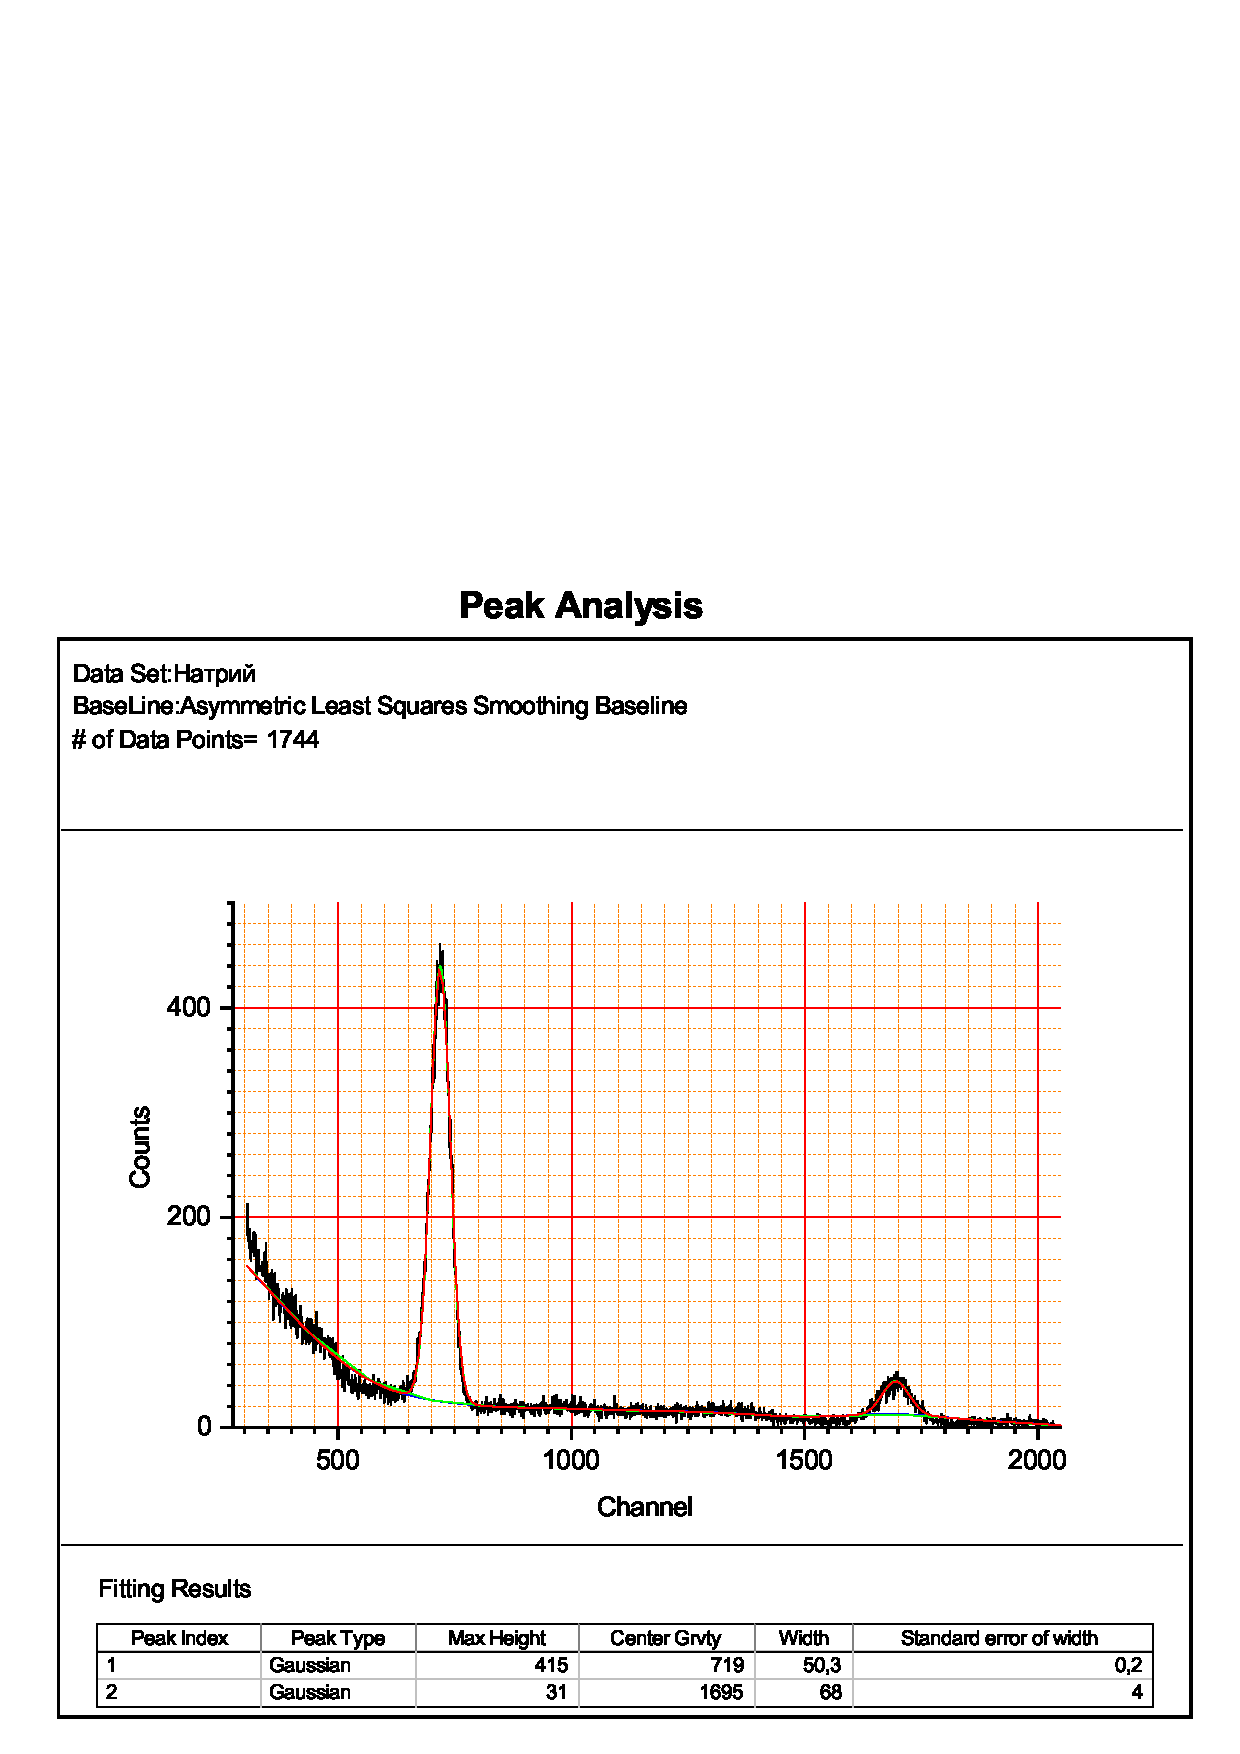
\includegraphics[width=0.8\textwidth]{1.png}
    \label{pic1}
\end{center}

Гадолиний является хорошим проводником электрического тока, a paбoчая частота генератора достаточно велика $(\sim 50$ к Гц $),$ поэтому для уменьшения вихревых токов образец изготовлен из мелких кусочков размером $\sim 0,5$ мм. Катушка 1 с образцом помещена в стеклянный сосуд 2, залитый трансформаторным маслом. Масло предохраняет образец от окисления и способствует
ухудшению электрического контакта между отдельными частичками образца. Кроме того, оно улучшает тепловой контакт между образцом и термостатируемой (рабочей) жидкостью 3 в термостате. Ртутный термометр 4 используется для приближённой оценки температуры.\\
При изменении температуры меняется магнитная восприимчивость образца $\chi,$ а следовательно, самоиндукция катушки и период колебаний $\tau$ автогенератора. Для измерения периода используется частотомер.
Закон Кюри Вейсса справедлив, если выполнено соотношение: 
\begin{equation*}
\frac{1}{\chi} \sim\left(T-\Theta_{p}\right) \sim \frac{1}{\left(\tau^{2}-\tau_{o}^{2}\right)}
\end{equation*}

где $\tau_{o}$ - период колебаний в отсутствие образца. Измерения проводятся в интервале температур от $12^{\circ} \mathrm{C}$ до $40^{\circ} \mathrm{C} .$ С целью
эКономии времени следует начинать измерения с низких температур.

Для охлаждения образца используется холодная водопроводная вода, циркулирующая вокруг сосуда с рабочей жидкостью (дистиллированной водой); рабочая жидкость постоянно перемешивается.

Величина стабилизируемой температуры задаётся на дисплее 5 термостата. Для нагрева служит внутренний электронагреватель, не показанный на
рисунке.

Когда температура рабочей жидкости в сосуде приближается к заданной, непрерывный режим работы нагревателя автоматически переходит в импульсный (нагреватель то включается, то выключается) - начинается процесс стабилизации температуры.

Температура исследуемого образца всегда несколько отличается от температуры дистиллированной воды в сосуде. После того как вода достигла
Заданной температуры, идёт медленный процесс выравнивания температур
образца и воды. Разность их температур контролируется с помощью медноконстантановой термопары 6 и цифрового вольтметра. Один из спаев термопары находится в тепловом контакте с образцом, а другой погружён в воду. Концы термопары подключены к цифровому вольтметру. Рекомендуется измерять период колебаний автогенератора в тот момент, когда указанная разность температур становится $\leqslant 0,5^{\circ} \mathrm{C} .$ Чувствительность термопары $\mathrm{K}=24$ град $/ \mathrm{мB}$


\section{Результаты измерений и их обработка}

Измерим зависимоть $\tau$ от температуры образца и занесем результаты в \textit{Таблицу \ref{data}}


\begin{table}[h!]
\begin{center}
\begin{tabular}{|l|l|l|l|l|}
\hline
$\tau$, мкс                          & $U$, мВ                          & $T_{гр}^{\circ} \mathrm{C}$      & $1 / (\tau^2 - \tau_0^2)$      & $T^{\circ} \mathrm{C}$      \\ \hline
10.154                               & -0.02                            & 12.0             & 0.0286                         & 11.95       \\ \hline
10.0868                              & -0.02                            & 14.02            & 0.0297                         & 13.97       \\ \hline
9.9702                               & -0.02                            & 16.02            & 0.0319                         & 15.97       \\ \hline
9.8791                               & -0.02                            & 17.11            & 0.0339                         & 17.06       \\ \hline
9.7815                               & -0.02                            & 18.0             & 0.0363                         & 17.95       \\ \hline
9.6377                               & -0.02                            & 19.01            & 0.0403                         & 18.96       \\ \hline
9.459                                & -0.02                            & 20.01            & 0.0468                         & 19.96       \\ \hline
9.0662                               & -0.019                           & 22.01            & 0.0709                         & 21.96       \\ \hline
8.7512                               & -0.02                            & 24.02            & 0.1178                         & 23.97       \\ \hline
8.6131                               & -0.02                            & 26.02            & 0.1642                         & 25.97       \\ \hline
8.5365                               & -0.02                            & 28.02            & 0.2094                         & 27.97       \\ \hline
8.4882                               & -0.02                            & 30.01            & 0.2529                         & 29.96       \\ \hline
8.4551                               & -0.02                            & 32.0             & 0.2947                         & 31.95       \\ \hline
8.4302                               & -0.02                            & 34.0             & 0.3364                         & 33.95       \\ \hline
8.4111                               & -0.02                            & 36.01            & 0.3772                         & 35.96       \\ \hline
8.3966                               & -0.02                            & 38.0             & 0.4154                         & 37.95       \\ \hline
8.3847                               & -0.02                            & 40.0             & 0.453                          & 39.95       \\ \hline
\multicolumn{2}{|l|}{$\sigma T_{true} \approx 0.02 + 0.03$^{\circ} \mathrm{C} = $0.05$^{\circ} \mathrm{C}} & \multicolumn{3}{l|}{$\delta 1 / (\tau^2 - \tau_0^2 )\approx 0.02$} \\ \hline
\end{tabular}
    \caption{Данные измерений}
    \label{data}
\end{center}
\end{table}
\begin{minipage}{.5\textwidth}
    \begin{tikzpicture}[scale=1]
    	\begin{axis}[
    		axis lines = left,
        	xlabel = {$T^{\circ} \mathrm{C}$},
        	ylabel = {$1 / (\tau^2 - \tau_0^2)$, $1/\mu s^2$},
        	ylabel style={red, scale=0.7},
        	xlabel style={red, scale=0.7},
        	%xmin=0, xmax=9,
        	title={Зависимость $1 / (\tau^2 - \tau_0^2)$ от $T$},
        	legend style={at={(0.03,-0.4)},anchor=west}
    		]
    		\addplot +[blue, only marks]  plot[
			error bars/.cd,
			x dir = both,
			x fixed = 0.1,
			y dir = both,
			y fixed relative=0.02,
		    ]
		    table[x=t_new, y=y, col sep=comma]{data.csv};
    		\addlegendentry{Экспериментальные точки};
    		\addplot [color=red, domain=18:40]{0.020975*x - 0.37912};
    		\addlegendentry{Линейная экстраполяция}

    	\end{axis}
    \end{tikzpicture}
\end{minipage}
\begin{minipage}{.5\textwidth}
    Построим график зависимости $1 / (\tau^2 - \tau_0^2)$ от $T$. Экстраполируем линейный участок зависимости, чтобы определить $\theta_p$ и $\theta_k$ для гадолиния.Находим:
    \begin{align*}
        \theta_p &= 18.1 \pm  0.2^{\circ} \mathrm{C}\\
        \theta_k &\approx 22 \pm 2^{\circ} \mathrm{C}
    \end{align*}
    Погрешность $\theta_p$ оценим через МНК линейной области. Погрешность $\theta_k$ оценим по близлижащим точкам. Сравнивая с табличным $\theta_{k\: tab} = 20.2^{\circ} \mathrm{C}$, видим, что значение попадает в доверительный интервал.
    
\end{minipage}

\section{Выводы}

Мы проверили закон Кюри-Вейсса вблизи точки Кюри и получили результаты, согласующиеся с теорией. Значение температуры Кюри совпало с табличным. 

\end{document}
